\documentclass[../lecture-notes.tex]{subfiles}

\begin{document}
Let
\[
	\{ (x_i, f_i )\}_{i=1}^N
\]
with $x_i \in \R^d$, $f_i \in \R$.

Aim: Find a ``nice'' function $f$ such that
\[
	f(x_i) = f_i \quad i = 1, \ldots, N
\]
To compute we need a discrete representation of $f$ in some basis
\[
	f(x) = \sum_{i=1}^N c_j b_j(x)
\]
For interpolation solve via
\[
	Bc = \hat{f},
\]
where $B_{ij} = b_j(x_i)$, $j = 1, \ldots, N$, $C = (C_1, \ldots, C_N)^\tp$.
If $B$ is a nonsingular we have a solution $\hat{f} = (f_1, \ldots, f_N)^\tp$.
It turns out that ``kernel'' functions which are entered at the $x_j$ are a good choice:
\[
	b_j(x) = K(x_j, x),
\]
so
\[
	f(x) = \sum_{j=1}^N c_j K(x_j, x).
\]
We will also consider $f(x_i) \approx f_i$.
\chapter{Kernel based methods} % Chapter 1
\label{sec:1}
\section{Kernels} % Section 1.1
\label{sec:1.1}
The Gaussian kernel is the prime example of a kernel:
\[
	K(x, y) \coloneqq \exp\left(- \alpha \| x - y \|_2^2 \right)
\]
for all $x, y \in \R^d$.
% Plot: Gaussian kernel for various alphas.
\begin{figure}[htpb]
\centering
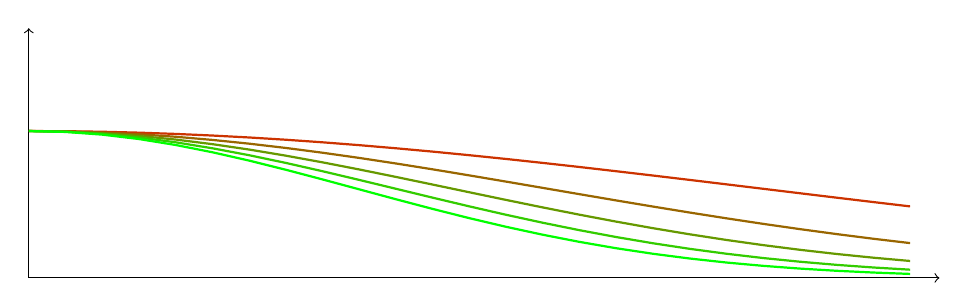
\begin{tikzpicture}[scale=\textwidth/6.5cm]
	\draw[->] (0, 0) -- (6.2, 0);
	\draw[->] (0,0) -- (0, 1.7);
	\foreach \a in {2, 4, ..., 10}
		\draw[domain=0:6, color=green!\a 0!red, thick] plot (\x, {exp(-\a*0.01*\x*\x)});
\end{tikzpicture}
\captionsetup{labelformat=empty}
\caption{Figure: Gaussian kernels for various $\alpha$ values}
\end{figure}
\begin{definition} % Definition 1
\label{thm:1}
Let $\Omega$ be an arbitrary nonempty set.
A function $K : \Omega \times \Omega \to \R$ is called a \keydef{kernel} on $\Omega$. We call $K$ a \keydef{symmetric kernel} if
\[
	K(x, y) = K(y, x)
\]
for all $x, y \in \Omega$.
\end{definition}
The Gaussian kernel can be written as
\begin{IEEEeqnarray*}{rCl}
	K(x, y) &=& \exp ( - \alpha \underbrace{ \| x-y \|_2^2 }_{r \coloneqq \| x - y \|_2}) \\
	&=& \exp(-\alpha r^2) \\
	&=& \phi(r) \\
	&=& \phi(\| x - y \|_2)
\end{IEEEeqnarray*}
\begin{definition} % Definition 2
\label{thm:2}
A function $\Phi : \R^d \to \R$ is said to be radial if there exists a function $\phi : [0, \infty] \to \R$ such that
\[
	\Phi(x) = \Phi(\| x \|_2)
\]
for all $x \in \R^d$.
Such functions are traditionally called \keydef{\acf{RBF}}.
\end{definition}
Other \ac{RBF}s are
\begin{itemize}
\item $\beta > 0$, multiquadratics, $\phi(r) = (1 + \alpha r^2)^\beta$ 
\begin{figure}[htpb]
\centering
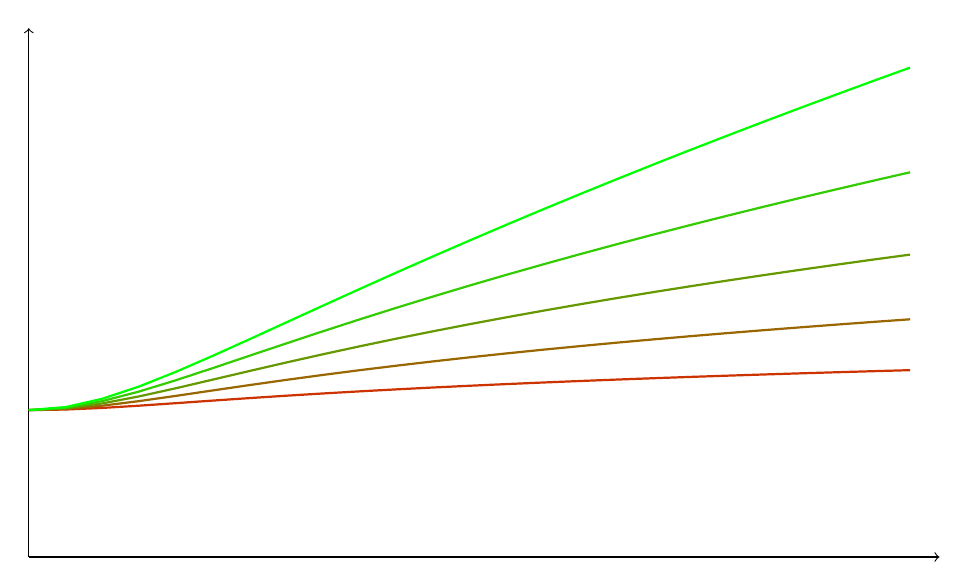
\begin{tikzpicture}[scale=\textwidth/6.5cm]
	\draw[->] (0, 0) -- (6.2, 0);
	\draw[->] (0,0) -- (0, 3.6);
	\foreach \a in {2, 4, ..., 10}
		\draw[domain=0:6, color=green!\a 0!red, thick] plot (\x, {pow(1 + \x*\x, \a/30)});
\end{tikzpicture}
\captionsetup{labelformat=empty}
\caption{Figure: Multiquadratics for various $\beta$ values}
\end{figure}
\item $\beta < 0$, inverse multiquadratics $\phi(r) = (1 + \alpha r^2)^\beta$
\begin{figure}[htpb]
\centering
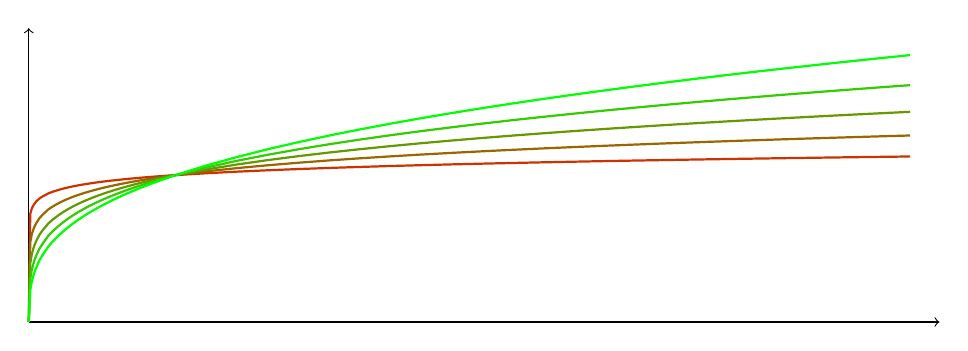
\begin{tikzpicture}[scale=\textwidth/6.5cm ]
	\draw[->] (0, 0) -- (6.2, 0);
	\draw[->] (0,0) -- (0, 2);
	\foreach \a in {2, 4, ..., 10}
		\draw[domain=0:1, color=green!\a 0!red, thick, samples=100] plot (\x, {pow(\x, \a/30)});
	\foreach \a in {2, 4, ..., 10}
		\draw[domain=1:6, color=green!\a 0!red, thick] plot (\x, {pow(\x, \a/30)});
\end{tikzpicture}
\captionsetup{labelformat=empty}
\caption{Figure: Inverse multiquadratics for various $\beta$ values}
\end{figure}
\item powers: $\phi(r) = r^\beta$, $\beta \notin 2 \Z$. These belong to the polyharmonic family of kernels:
\[
	\phi(r) = r^\beta \log(r), \quad \beta \in 2 \Z.
\]
Special case:
\[
	\phi(r) = r^2 \log (r).
\]
This is the thin-plate spline.
\end{itemize}
% Plot: Inverse multiquadratics for various beta.
% Plot: Multiquadratics for various beta.
Wendland's kernel is a compactly supported kernel:
\[
	\phi_{3, 1}(r) = (1-r)^4_{+} (1 + 4r)
\]
with the cut-off function
\[
	(x)_+ \coloneqq \begin{cases}
		x, & x \geq 0 \\
		0, & x < 0
	\end{cases}
\]
\begin{remark}
Kernels can always be restricted to subsets without losing essential properties. This easily allows kernels on embedded manifolds, e.g.\ the sphere.
\end{remark}
\begin{remark}
We will see that a kernel $K$ on $\Omega$ defines a function $K(x, \cdot)$ for all fixes $x \in \Omega$.
The space
\[
	\mathcal{K}_0 \coloneqq \spn \left\{ K(x, \cdot) \mid x \in \Omega \right\}
\]
can be used as trial space in meshless methods for solving PDEs.
\end{remark}
In machine learning one views the kernel as a similarity measure
\[
	K : \Omega \times \Omega \to \R
\]
returns a number $K(x, y)$ describing the similarity of $x$ and $y$.
In $\R^d$,
\[
	\langle x, y \rangle = \sum_{i=1}^d x_i \cdot y_i.
\]
$x$ and $y$ are very dissimilar if they are orthogonal and $x$ and $y$ are very similar if they point in the same direction.

To work with general data, we first represent it in a Hilbert space $\spF$, the so called \keydef{feature space}.
One considers the feature map
\[
	\Phi : \Omega \to \spF.
\]
We can use the scalar product in $\spF$,
\[
	\langle \Phi(x), \Phi(y) \rangle_{\spF} \eqqcolon K(x, y) \quad \text{for all } x, y \in \Omega
\]
and define a kernel that way.

Consider a collection of documents. We represent it as a bag of words and describe a bag as a vector in a space where each dimension is associated with a word from the dictionary.
The feature map is
\[
	\Phi(t) \coloneqq \left(wf(w_1, t), wf(w_2, t), \ldots, wf(w_d, t) \right) \in \R^d
\]
where $wf(w_i, t)$ is the frequency of the word $w_i$ in the document $t$.
A simple kernel is the vector space kernel
\[
	K(t_1, t_2) \coloneqq \langle \Phi(t_1), \Phi(t_2) \rangle = \sum_{j=1}^d wf(w_j, t_1) \cdot wf(w_j, t_2).
\]
Natural extensions to this kernel take e.g.\ word order, relevance or semantics into account, which can be achieved by using matrices in the scalar product:
\begin{IEEEeqnarray*}{rCl}
	K(t_1, t_2) &\coloneqq& \langle S \Phi(t_1), S \Phi(t_2) \rangle \\
	&=& \Phi^\tp(t_1) S^\tp S \Phi(t_2).
\end{IEEEeqnarray*}
\end{document}